\section{Simulation Evaluation}
\label{sec:evaluation}

The simulations are conducted on a personal computer with an Intel(R) Core(TM) Ultra 9 185H CPU and NVIDIA GeForce RTX 4060 Max-Q / Mobile GPU, utilizing ROS2. To accelerate computation, particle processing was parallelized using CUDA. All experiments were conducted with a network of 20 agents (nodes), using a total of 2000 particles distributed evenly with 100 particles per agent.

To begin, Figure~\ref{fig:gt_messy_comparison} illustrates the challenge posed by outlier-rich environments.
Figure~\ref{fig:gt_graph} shows the ground truth pose graph. In contrast, Figure~\ref{fig:messy_graph} depicts a scenario where 40\% of the edges are incorrect due to outliers. In such an environment, optimization-based methods like DPGO can fail to converge to the correct solution, as demonstrated by the distorted graph. This highlights the need for robust methods capable of handling significant numbers of outliers.

\begin{figure}[H]
    \centering
    \subfloat[Ground Truth Pose Graph\label{fig:gt_graph}]{%
        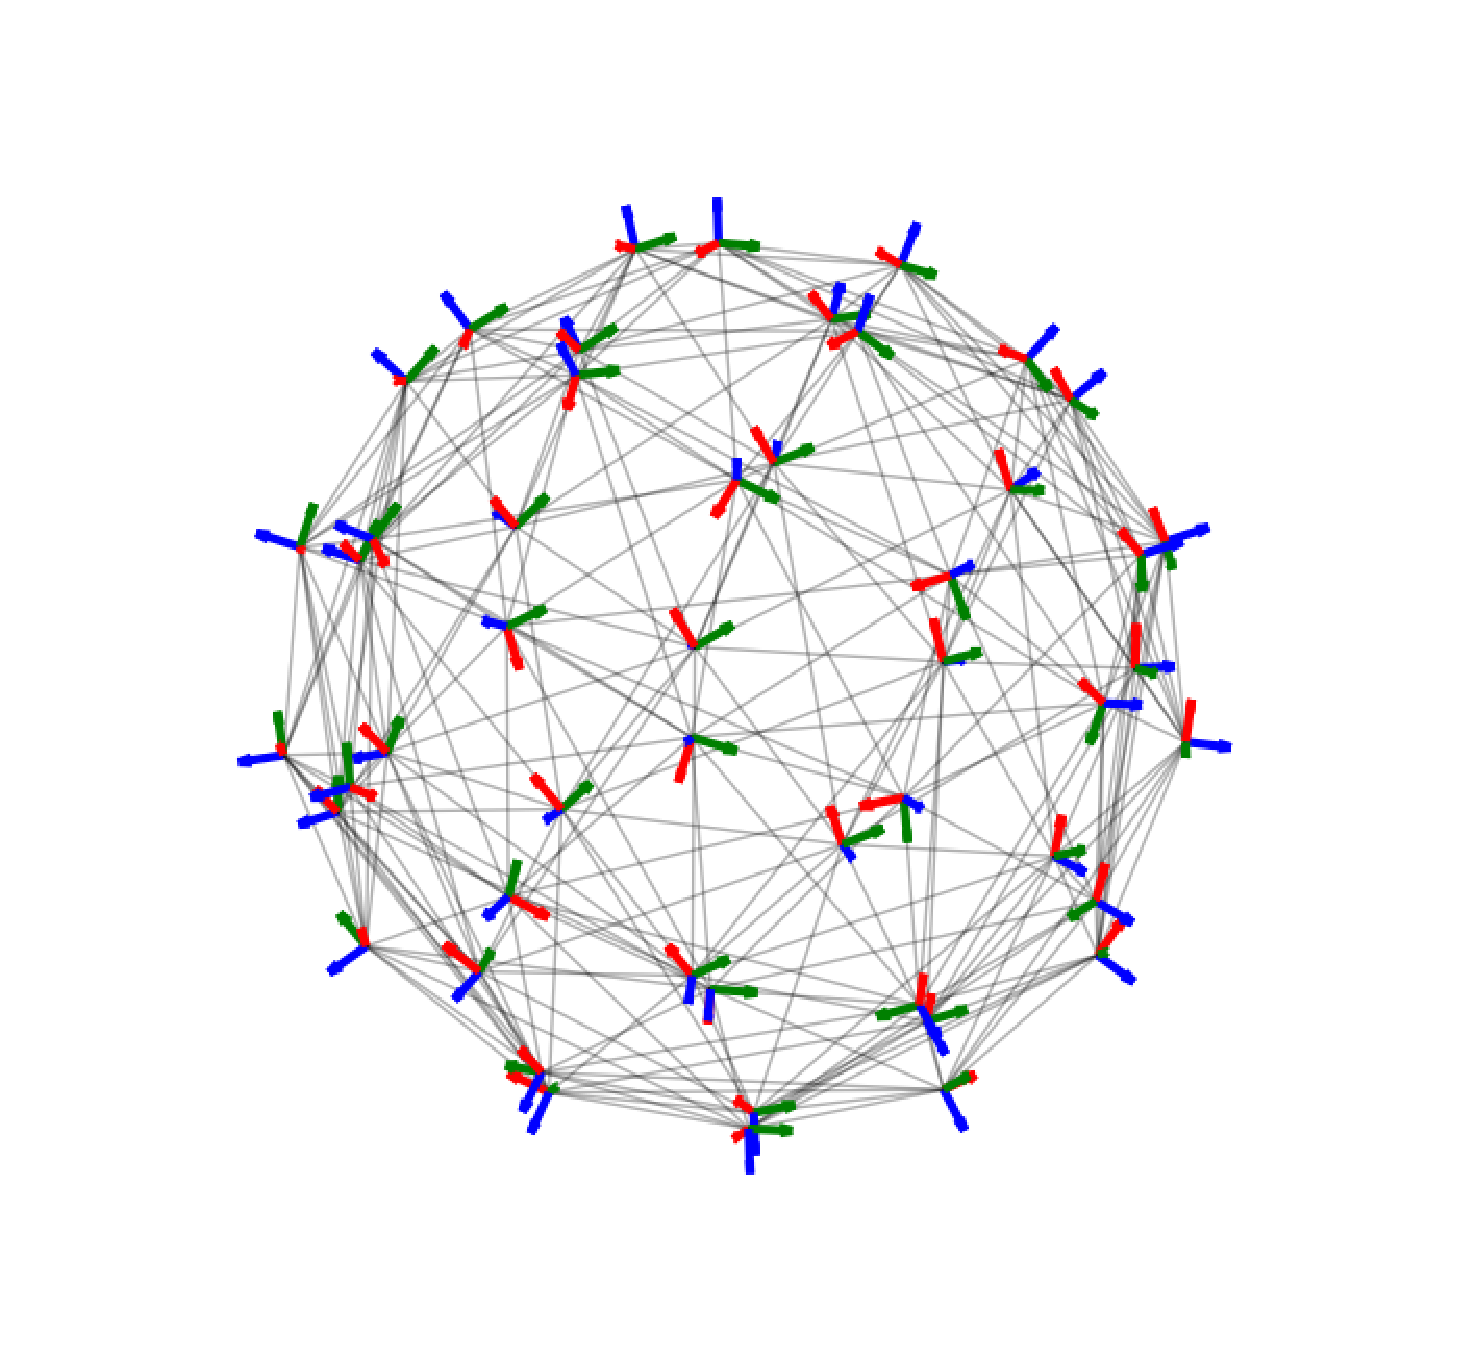
\includegraphics[width=0.45\linewidth]{fig/gt_graph.eps}%
    }
    \hfill
    \subfloat[DPGO result in an outlier environment (40\% incorrect edges)\label{fig:messy_graph}]{%
        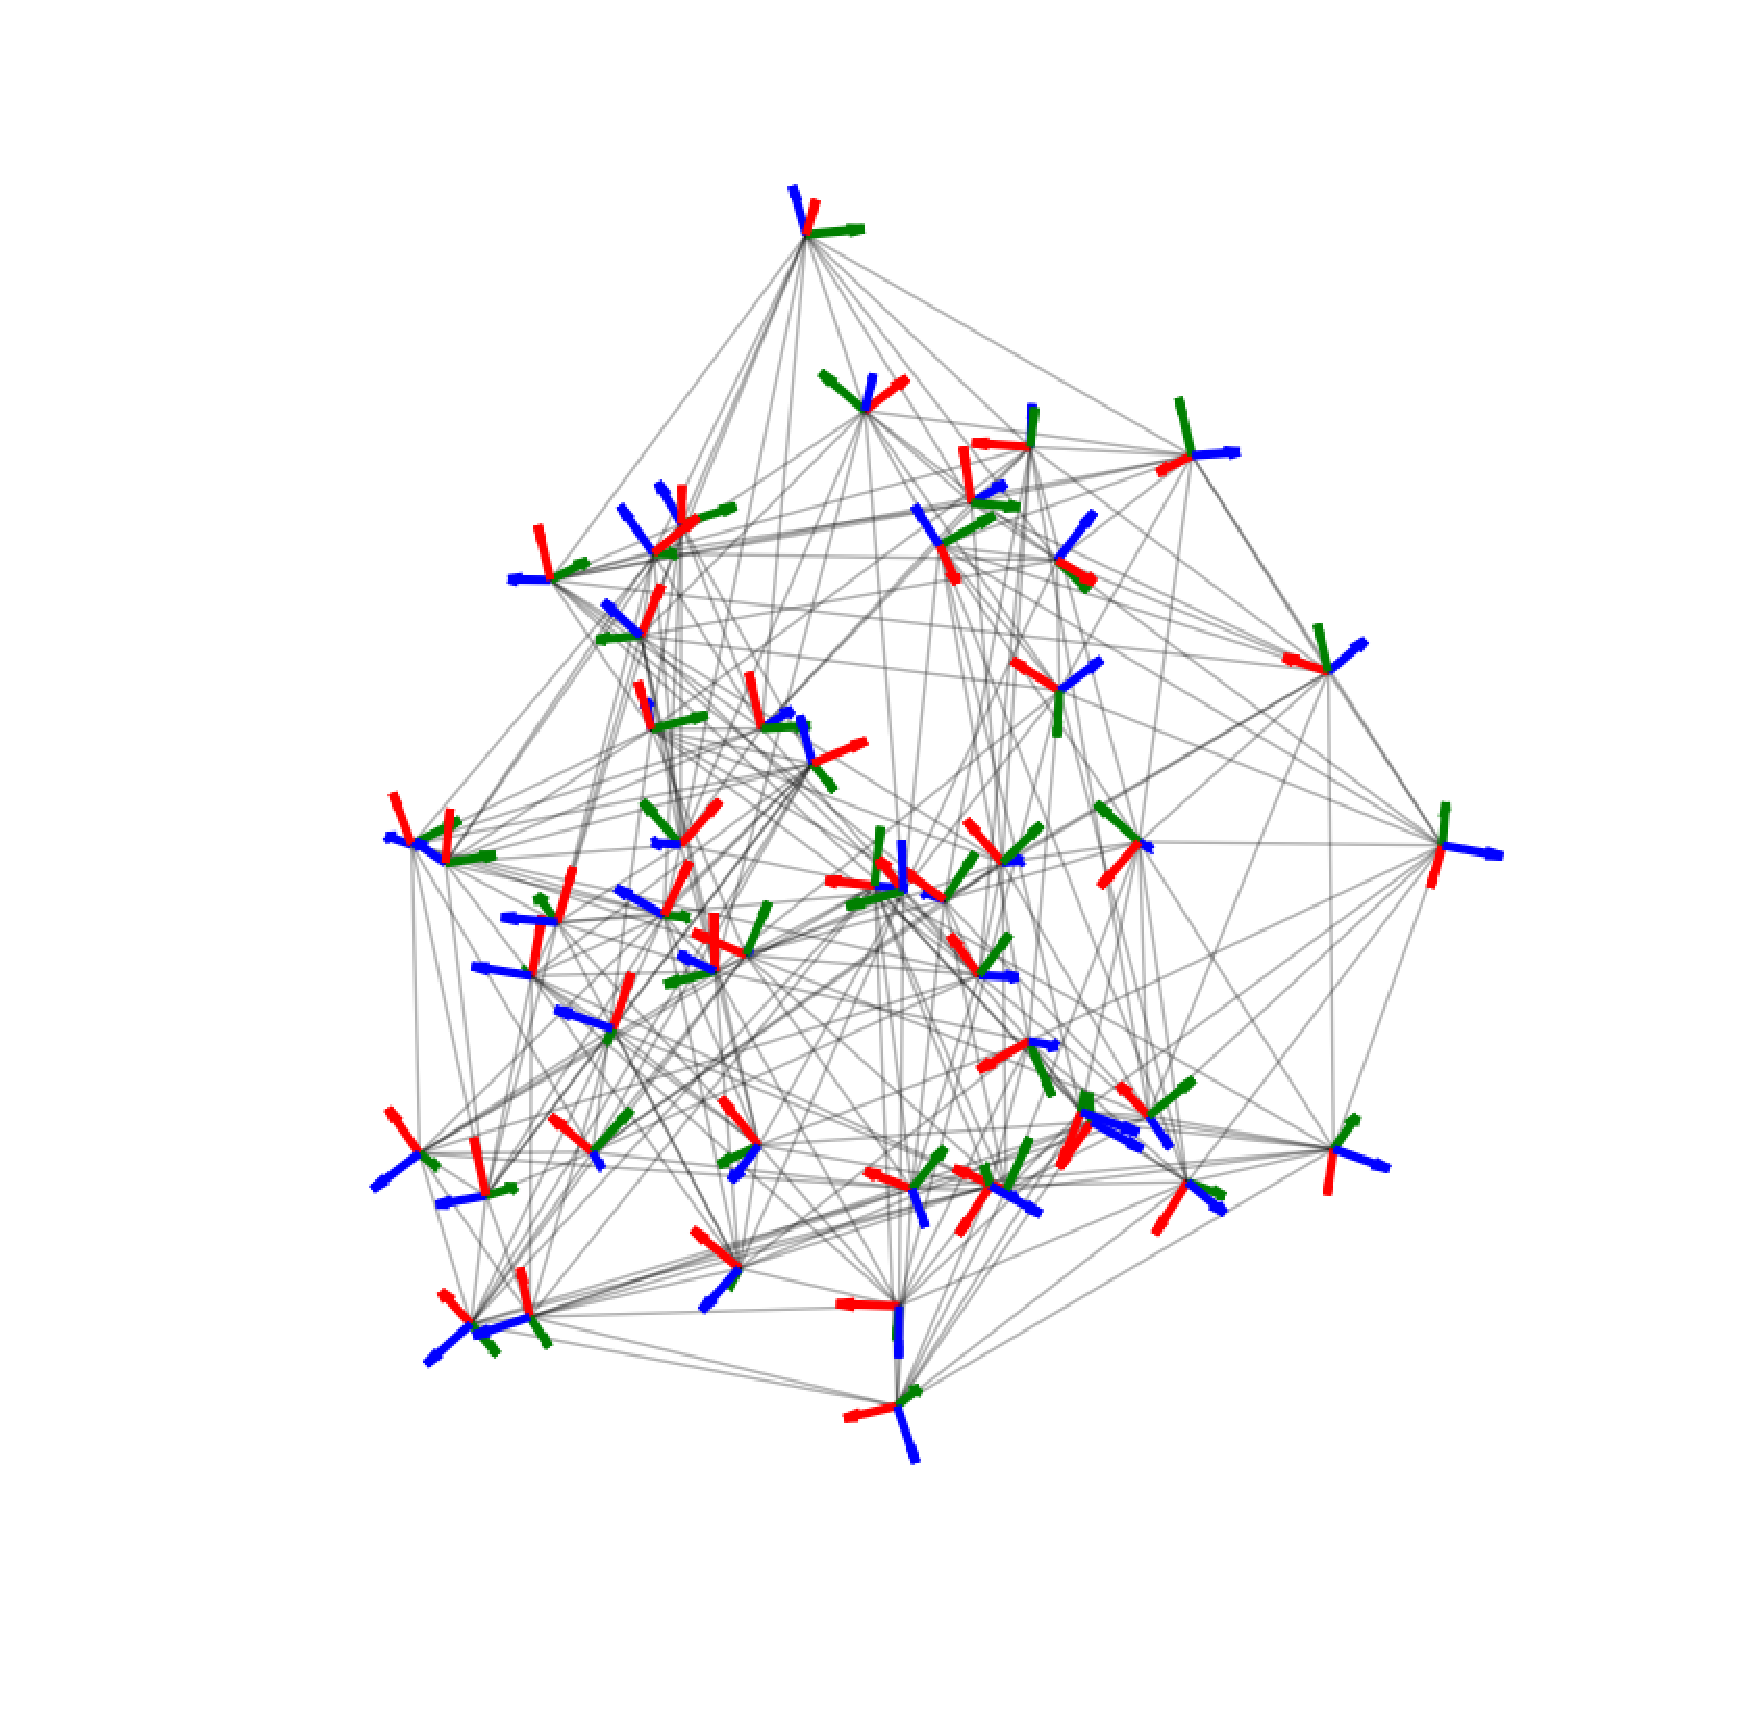
\includegraphics[width=0.45\linewidth]{fig/messy_graph.eps}%
    }
    \caption{Comparison of ground truth and DPGO performance in an outlier-rich environment.}
    \label{fig:gt_messy_comparison}
\end{figure}

In this section, we further evaluate the performance of the proposed method in environments with and without outliers.
We compare our method with the proposed method using Gauss-Newton optimization, and Distributed Certifiably Correct Pose-Graph Optimization (DPGO)~\cite{Tian2021}.

\subsection{Environment without Outliers}
\label{subsec:eval_no_outliers}

Figures~\ref{fig:no_outliers_graphs_1} and \ref{fig:no_outliers_graphs_last} show the pose graphs before and after optimization, respectively.
Figure~\ref{fig:no_outliers_edge_errors} shows the time transition of the edge cost $c_{ij}$, and Figure~\ref{fig:no_outliers_particle_variances} shows the time transition of the particle variance for each agent.
Specifically, Figure~\ref{fig:no_outliers_edge_errors} displays the range (shaded area) between the minimum and maximum costs across all connected edges, along with their mean value.
Figure~\ref{fig:no_outliers_particle_variances} similarly shows the range (shaded area) of particle variances across all agents, and their mean value.

\begin{figure}[H]
    \centering
    \subfloat[Before optimization\label{fig:no_outliers_graphs_1}]{%
        \includegraphics[width=0.45\linewidth]{fig/graph_temp_step_1.eps}%
    }
    \hfill
    \subfloat[After optimization\label{fig:no_outliers_graphs_last}]{%
        \includegraphics[width=0.45\linewidth]{fig/graph_temp_step_last.eps}%
    }
    \\
    \subfloat[Edge errors $c_{ij}$\label{fig:no_outliers_edge_errors}]{%
        \includegraphics[width=0.45\linewidth]{fig/edge_errors_temp.eps}%
    }
    \hfill
    \subfloat[Particle variances\label{fig:no_outliers_particle_variances}]{%
        \includegraphics[width=0.45\linewidth]{fig/particle_variances_temp.eps}%
    }
    \caption{Evaluation in an environment without outliers.}
    \label{fig:eval_no_outliers}
\end{figure}

\subsection{Environment with Outliers}
\label{subsec:eval_with_outliers}

In this subsection, we evaluate the performance in an environment with outliers. In this outlier validation (corresponding to Figure~\ref{fig:eval_with_outliers}), incorrect edges are selected at a rate of 0.3 in each step.
Figures~\ref{fig:with_outliers_graphs_1} and \ref{fig:with_outliers_graphs_last} show the pose graphs before and after optimization in an environment with outliers.
Figure~\ref{fig:with_outliers_edge_errors} shows the time transition of the edge cost $c_{ij}$, and Figure~\ref{fig:with_outliers_particle_variances} shows the time transition of the particle variance for each agent.
Specifically, Figure~\ref{fig:with_outliers_edge_errors} displays the range (shaded area) between the minimum and maximum costs across all connected edges, along with their mean value. It shows that although errors occur, they do not diverge and maintain a certain level.
Figure~\ref{fig:with_outliers_particle_variances} similarly shows the range (shaded area) of particle variances across all agents, and their mean value, indicating that outliers cause an increase in particle variance.

\begin{figure}[H]
    \centering
    \subfloat[Before optimization\label{fig:with_outliers_graphs_1}]{%
        \includegraphics[width=0.45\linewidth]{fig/graph_temp2_step_1.eps}%
    }
    \hfill
    \subfloat[After optimization\label{fig:with_outliers_graphs_last}]{%
        \includegraphics[width=0.45\linewidth]{fig/graph_temp2_step_last.eps}%
    }
    \\
    \subfloat[Edge errors $c_{ij}$\label{fig:with_outliers_edge_errors}]{%
        \includegraphics[width=0.45\linewidth]{fig/edge_errors_temp2.eps}%
    }
    \hfill
    \subfloat[Particle variances\label{fig:with_outliers_particle_variances}]{%
        \includegraphics[width=0.45\linewidth]{fig/particle_variances_temp2.eps}%
    }
    \caption{Evaluation in an environment with outliers.}
    \label{fig:eval_with_outliers}
\end{figure}

% \subsection{Benchmark Results}
% \label{subsec:benchmark_results}

In the benchmark comparisons, for DPGO, an optimization problem with incorrectly selected edges based on each outlier ratio is solved. For the proposed method (ASP-PGF), edges are randomly misselected at each of the 50 steps based on the outlier ratio. As demonstrated in our experiments, the algorithm consistently converges to a KKT point (as proven in Theorem 4.1) within 50 iterations in our 20-agent, 1000-particle scenario, confirming the theoretical guarantees.

Table~\ref{tab:benchmark_results} summarizes the performance metrics for each method.
As the outlier ratio increases, the filtering-based proposed method (ASP-PGF) surpasses the accuracy of optimization-based methods like DPGO.

\begin{table}[H]
  \centering
  \caption{Benchmark Results (Single Metric)}
  \label{tab:benchmark_results}
  \begin{tabular}{@{}lccc@{}}
    \toprule
    Environment & DPGO~\cite{Tian2021} & ASP-PGF(GN) \\
    \midrule
    Without Outliers & \textbf{1.10}\times 10^{-11} & 0.026 \\
    Outlier Ratio 0.2 & \textbf{0.216} & 0.591 \\
    Outlier Ratio 0.4 & 0.902 & \textbf{0.742} \\
    \bottomrule
  \end{tabular}
\end{table}
